%%%%%%%%%%%%%%%%%%%%%%%%%%%%%%%%%%%%%%%%%%%%%%%%%%%%%%%%%%%%%%%%%%%%%
%
% CSCI 1430 Writeup Template
%
% This is a LaTeX document. LaTeX is a markup language for producing
% documents. Your task is to fill out this
% document, then to compile this into a PDF document.
%
% TO COMPILE:
% > pdflatex thisfile.tex
%
% For references to appear correctly instead of as '??', you must run
% pdflatex twice.
%
% If you do not have LaTeX and need a LaTeX distribution:
% - Departmental machines have one installed.
% - Personal laptops (all common OS): www.latex-project.org/get/
%
% If you need help with LaTeX, please come to office hours.
% Or, there is plenty of help online:
% https://en.wikibooks.org/wiki/LaTeX
%
% Good luck!
% James and the 1430 staff
%
%%%%%%%%%%%%%%%%%%%%%%%%%%%%%%%%%%%%%%%%%%%%%%%%%%%%%%%%%%%%%%%%%%%%%
%
% How to include two graphics on the same line:
%
% \includegraphics[\width=0.49\linewidth]{yourgraphic1.png}
% \includegraphics[\width=0.49\linewidth]{yourgraphic2.png}
%
% How to include equations:
%
% \begin{equation}
% y = mx+c
% \end{equation}
%
%%%%%%%%%%%%%%%%%%%%%%%%%%%%%%%%%%%%%%%%%%%%%%%%%%%%%%%%%%%%%%%%%%%%%%%%%%%%%%%%%%%%%%%%%%%%%%%%

\documentclass[11pt]{article}

\usepackage[english]{babel}
\usepackage[utf8]{inputenc}
\usepackage[colorlinks = true,
            linkcolor = blue,
            urlcolor  = blue]{hyperref}
\usepackage[a4paper,margin=1.5in]{geometry}
\usepackage{stackengine,graphicx}
\usepackage{fancyhdr}
\setlength{\headheight}{15pt}
\usepackage{microtype}
\usepackage{times}
\usepackage{booktabs}

% python code format: https://github.com/olivierverdier/python-latex-highlighting
\usepackage{pythonhighlight}

\frenchspacing
\setlength{\parindent}{0cm} % Default is 15pt.
\setlength{\parskip}{0.3cm plus1mm minus1mm}

\pagestyle{fancy}
\fancyhf{}
\lhead{Project 2 Writeup}
\rhead{CSCI 1430}
\rfoot{\thepage}

\date{}

\title{\vspace{-1cm}Project 2 Writeup}


\begin{document}
\maketitle
\vspace{-2cm}
\thispagestyle{fancy}

% \section*{Instructions}
% \begin{itemize}
%   \item This write-up is intended to be `light'; its function is to help us grade your work.
%   \item Please describe any interesting or non-standard decisions you made in writing your algorithm.
%   \item Show your results and discuss any interesting findings.
%   \item List any extra credit implementation and its results.
%   \item Feel free to include code snippets, images, and equations.
%   \item Use as many pages as you need, but err on the short side.
%   \item \textbf{Please make this document anonymous.}
% \end{itemize}

\section*{Project Overview}

In this project, feature matching is implemented in the following steps:

\begin{itemize}
    \item Implement function \verb|get_features()| to get SIFT like features
    \item Implement function \verb|match_features()| for matching features
    \item Implement function \verb|get_interest_points()| to get interest points using Harris cornes detection.
\end{itemize}

\section*{Implementation Detail}
 
The implementation order is follwing the implementation strategy part on \href{https://browncsci1430.github.io/webpage/proj2_featurematching/}{project website}. The accuracy results will be discussed in the Results section.

\subsection*{Explaination for implementation of get\_features()}

At first, an error message will be raised if the feature width is not a multiple of 4. And then to improve the accuracy, especially for EpiscopalGaudi case, the image is rescaled if the input image is too small. The corresponding interest points are also rescaled to the same factor. The same operation has also been done in \verb|get_interest_points()| function. This one operation can increase accuracy on EpiscopalGaudi from 10\% to 80\%.

For each interested points, a box with the shape of [feature\_width, feature\_width] around the interest point is cut out for feature construction. Interested ponts that are close to the image edge will be skipped. The window is then splitted into cells with the shape of [4, 4]. Each cell will be reprensented by a one dimension feature with length 8, the value of which is calculated by summing up magnitude of the gradients of pixels in specific orientation. Then one feature for the whole window is obtained by concatenating all cell features, resulting in a one dimension vector with length as 128 for one interest point. The feature vector is normalized and clipped by a threshold and then renormalized before collected by \verb|features|.

Two different descriptors are also implemented and their implementation and performance are discussed in the Extra Credits section.

\subsection*{Explaination for  implementation for match\_features()}

The feature vectors for interest points from two images are compared similarity by calculating Euclidean distances among all pairs. The shortest the distance is, the more similar the two points are. The confidence value is defined as 1 - nddr. To improve the accuracy, the matches has been performed from image2 to image1 as well as from image1 to image2. And the common pairs are extracted for the final matches. This can increase accuracy from 80\% to 90\% or so. PCA analysis has been implemented for test purpose and are discussed in the Extra Credit section.

\subsection*{Explaination for implementation for get\_interest\_points()}

At first, the image is also rescaled the same as it stated in \verb|get_features()| function. However, the returned x and y coordinates are rescaled back to the original input shape to avoid conflicting the \verb|main.py|. Then, the image is filtered with gaussian filter for better detection. The gradients for each pixels are calculated using \verb|np.gradient()|. And the $R$ values are calculated using \(R = det(M) - \alpha(trace(M))\), where \(\alpha = 0.04\). The $R$ is then normalized to unit length and clipped the smallest 15\% value to 0. Interest points are picked using \verb|feature.peak_local_max()| function, which pick the largest value among a window size of \verb|feature_width//2| * \verb|feature_width//2|.

\section*{Result}

Results for NotreDame, MountRushmore and EpiscopalGaudi pairs are presented below. The program is run in local with the same python environment on the department machine. The results are obtained with the optimal hyperparameters, SIFT-like descriptor and rescaling operation for images that are too small. The However, I found that there might be 1\% accuracy difference from the results on Gradescope.

\begin{enumerate}
    \item NotreDame:
    \begin{itemize}
        \item Matches: 380
        \item Accuracy on 50 most confident: 100\%
        \item Accuracy on 100 most confident: 100\%
        \item Accuracy on all matches: 68\%
    \end{itemize}
    
    \begin{figure}[htbp]
        \centering
        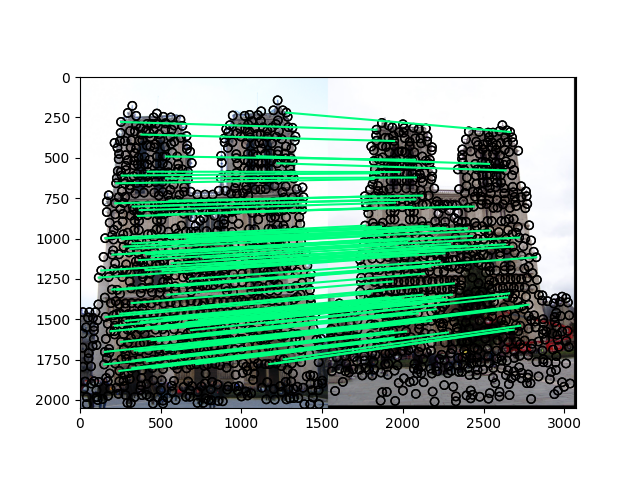
\includegraphics[scale=0.8]{../results/notre_dame_matches.png}
        \caption{Mathces on 100 most confident pairs of NotreDame}
        \label{notredame}
    \end{figure}

    \item MountRushmore:
    \begin{itemize}
        \item Matches: 737
        \item Accuracy on 50 most confident: 100\%
        \item Accuracy on 100 most confident: 100\%
        \item Accuracy on all matches: 56\%
    \end{itemize}
    
    \begin{figure}[htbp]
        \centering
        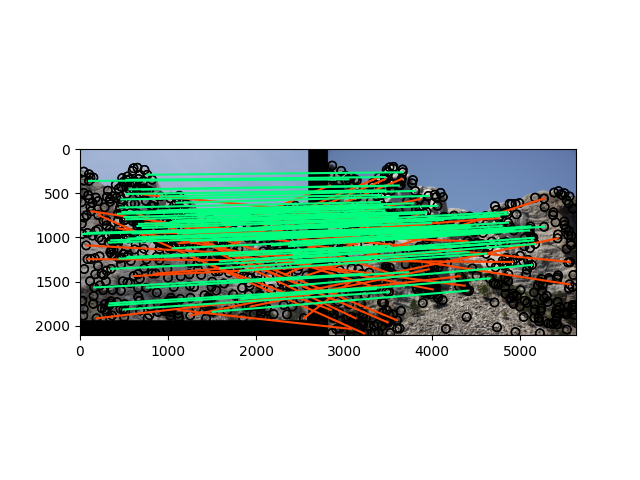
\includegraphics[scale=0.8]{../results/mt_rushmore_matches.png}
        \caption{Mathces on 100 most confident pairs of MountRushmore}
        \label{mountrushmore}
    \end{figure}

    \item EpiscopalGaudi:
    \begin{itemize}
        \item Matches: 495
        \item Accuracy on 50 most confident: 94\%
        \item Accuracy on 100 most confident: 88\%
        \item Accuracy on all matches: 44\%
    \end{itemize}
    
    \begin{figure}[htbp]
        \centering
        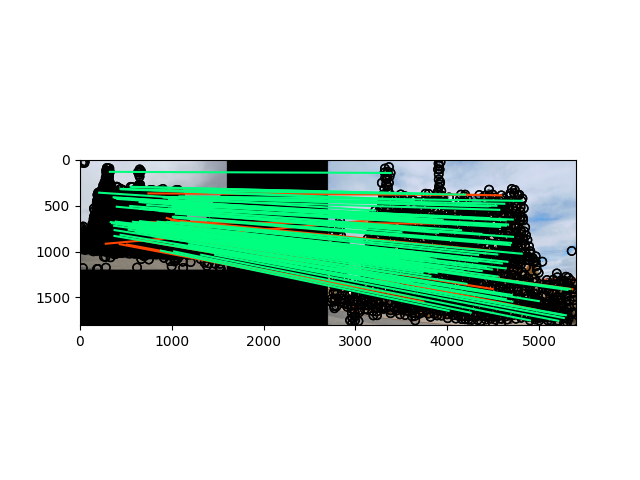
\includegraphics[scale=0.8]{../results/e_gaudi_matches.png}
        \caption{Mathces on 100 most confident pairs of EpiscopalGaudi}
        \label{mountrushmore}
    \end{figure}

\end{enumerate}

% \begin{figure}[h]
%     \centering
%     
\includegraphics[width=5cm]{placeholder.jpg}
%     
\includegraphics[width=5cm]{placeholder.jpg}
%     \caption{\emph{Left:} My result was spectacular. \emph{Right:} Curious.}
%     \label{fig:result1}
% \end{figure}

\section*{Extra Credit (Optional)}
\begin{enumerate}
    \item \textbf{Detection}
    
    Adaptive non-maximum suppression (ANMS) implementation
    The ANMS is implemented in the following manner: distances between the point $A$ and the nearest point of which 90\% R value is larger than the point $A$ are calculated and sorted. Only the first 500 points with the largest distance value are extracted as interest points. In this way, we could suppress points that close the the peak we pick but with small R value.

    The results with ANMS implementation are presented below. Compared to the results in Result section, we found the accuracy for all three cases decreases. The decrease here might be the number of points we pick here is only 500 while before ANMS, the number of points varies from 700 to 2000. To sum up, this method might be useful in some case but it doesn't show better performance here.
    \begin{itemize}
        \item NotreDame:  
            \begin{itemize}
                \item Matches: 206
                \item Accuracy on 50 most confident: 100\%
                \item Accuracy on 100 most confident: 93\%
                \item Accuracy on all matches: 57\%
            \end{itemize}
        \item MountRushmore:  
            \begin{itemize}
                \item Matches: 211
                \item Accuracy on 50 most confident: 96\%
                \item Accuracy on 100 most confident: 65\%
                \item Accuracy on all matches: 36\%
            \end{itemize}
        \item MountRushmore:  
            \begin{itemize}
                \item Matches: 165
                \item Accuracy on 50 most confident: 68\%
                \item Accuracy on 100 most confident: 40\%
                \item Accuracy on all matches: 26\%
            \end{itemize}
    \end{itemize}
   
    
    Here is the corresponding part code in the implementation.
    \begin{python}
def anms(points, R, top=500):
    l, x, y = [], 0, 0
    threshold = np.mean(R)
    while x < len(points):
        minpoint = float("inf")
        xi, yi = points[x][0], points[x][1]
        while y < len(points):
            xj, yj = points[y][0], points[y][1]
            if (
                xi != xj
                and yi != yj
                and R[points[x][0], points[x][1]] > threshold
                and R[points[y][0], points[y][1]] > threshold
                and R[points[x][0], points[x][1]]
                < R[points[y][0], points[y][1]] * 0.9
            ):
                dist = math.sqrt((xj - xi) ** 2 + (yj - yi) ** 2)
                if dist < minpoint:
                    minpoint = dist
            y += 1
        l.append([xi, yi, minpoint])
        x += 1
        y = 0
    l.sort(key=lambda x: x[2], reverse=True)
    return np.array(l[:top])
    \end{python}
\newpage
    \item \textbf{Description}:
    \begin{itemize}
        \item It have been tested with \textbf{different number of bins}. The accuracy with different number of bins is presented below. (The accuracy on 100 most confident matches for NotreDame is run in local, which might have less than 1 \% difference from results on Gradescope. All other parameters are values shown in code.) From the table, we could see that tt can harm the accuracy if the number of bins is too small but won't change the accuracy too much if the number is enough. However, the excution time will increase with the increase of the number of bins. Thus, 8 is suitable for descriptor construction considering both accuracy and excution time.
       
        \begin{table}[htbp]
            \centering
            \begin{tabular}{c c c c c c c c}
                \toprule
            Number of bins & 4 & 6 & 8 & 10 & 12 & 30 \\
                \midrule
            Accuracy & 94 & 97 & 100 & 99 & 99 & 99 \\
            Excution Time (s) & 5.58 & 5.91 & 6.13 & 6.74 & 8.30  & 14.93 \\
                \bottomrule
            \end{tabular}
            \caption{Accuracy changes w.r.t the number of bins on NotreDame case. (Excution time is measured in local.)}
        \label{bin_number}
        \end{table}


       \item \textbf{Different spatial layouts for feature}: 
       There are two other types of descriptors have been implemented. The type can be chosen through one parameter \verb|descriptor_type| in \verb|get_features()| function.
       \begin{itemize}
        \item \textbf{HOG-like descriptor}: the main idea is that the gradient closer to the center orientation of the corresponding bins will contribute more to the bin value. Thus, the contribution is calculated using
       
        \[ value = \sum_i magnitude_i * \frac{orientation_i - center}{bin\_width} \]
        
         However, though the construction of feature has taken the orientation of gradient into consideration, the accuracy on 100 most confident matches for NotreDame decreases from 100\% to 99\%. And for MountRushmore is the same. However, for EpiscopalGaudi, the accuracy increase from 88\% to 90\%.
 
         Here is the corresponding part code in the implementation.
        \begin{python}
 for subwindow_i in range(len(patch_window_magnitudes)):
     inds = np.digitize(patch_window_orientations[subwindow_i], bins)
     for inds_i in range(num_bins):
         mask = np.array(inds == inds_i)
         feature[subwindow_i * num_bins + inds_i] = np.dot(
         patch_window_magnitudes[subwindow_i].flatten()[mask],
         np.cos(
             np.abs(
             patch_window_orientations[subwindow_i].flatten()[mask]
                 - (bins[inds_i] + bin_width / 2)
                 )
             ),
         )
         \end{python}
 
         \item \textbf{GLOH-like descriptor}: borrows the idea from the GLOH descriptor. In the cell, pixels are firstly grouped based upon their orientation and then grouped pixels are grouped based upon their magnitude again, which results in 24 bins for one cell. Thus, the total feature length is 384. This is GLOH-like descriptor as I have not fully understand how to implement the true GLOH descriptor. This descriptor also increase the accuracy on EpiscopalGaudi to 90\%.


         Here is the corresponding part code in the implementation.
         \begin{python}
mag_bin = np.array([0,2,4])
for subwindow_i in range(len(patch_window_magnitudes)):
    inds = np.digitize(patch_window_orientations[subwindow_i], bins)
    for inds_i in range(num_bins):
        mask = np.array(inds == inds_i)
        sub_inds = np.digitize(
        patch_window_magnitudes[subwindow_i][mask], mag_bins
            )
        for sub_inds_i in range(num_mag_bins):
            sub_mask = np.array(sub_inds == sub_inds_i)
            feature.append(
            np.dot(
            patch_window_magnitudes[subwindow_i].flatten()[mask][
                            sub_mask],
            np.cos(
            np.abs(
            patch_window_orientations[subwindow_i].flatten()[
                    mask][
                            sub_mask]
                    - (bins[inds_i] + bin_width / 2)
                            )
                        ),
                    )
                )
         \end{python}
        
       \end{itemize} 
   \end{itemize}
\newpage
   \item \textbf{Matching}: Principle component analysis (PCA) implementation
   
   The PCA method has been implemented as following. The idea of PCA is analyzing the weight of each feature component and project it onto those dimensions with larger wights. In default of current implementation, the first 32 components are extracted for matching. However, the accuracy decreases to 0 - 2\%. (I have checked with \verb|sklearn.decomposition.PCA()|, which shows the same result.)
   \begin{python}
def PCA(features, m=32):
    C = features - np.mean(features, axis=0)
    cov_matrix = np.cov(C.T)
    eigenvals, eigenvecs = np.linalg.eig(cov_matrix)
    i = np.argsort(-1 * np.abs(eigenvals))
    eigenvecs = eigenvecs[i]
    eigenvals = eigenvals[i]
    pca_features = np.dot(eigenvecs.T, C.T)
    return pca_features[:m].T
   \end{python}

\end{enumerate}

\end{document}
